\documentclass[conference]{IEEEtran}
\IEEEoverridecommandlockouts
% The preceding line is only needed to identify funding in the first footnote. If that is unneeded, please comment it out.
%Template version as of 6/27/2024

%\usepackage{cite}
\usepackage{amsmath,amssymb,amsfonts}
\usepackage{algorithmic}
\usepackage{graphicx}
\usepackage{textcomp}
\usepackage{xcolor}
\def\BibTeX{{\rm B\kern-.05em{\sc i\kern-.025em b}\kern-.08em
    T\kern-.1667em\lower.7ex\hbox{E}\kern-.125emX}}
    

\definecolor{dg}{RGB}{64,64,64}

\usepackage[colorlinks = true,
		citecolor = black,
		urlcolor= blue,
		linkcolor=dg,]{hyperref}

\begin{document}

\title{Evaluating Progress in Web3 Grants: Introducing the Grant Maturity Index.
\thanks{This work is has been funded by the EU in the framework of the NGI TRUSTCHAIN project under the European Commission HORIZON-CL4-2022-HUMAN-01-03 grant: \href{https://cordis.europa.eu/project/id/101093274}{101093274} and by \href{https://ens.domains/}{ENS Domains} through its \textit{Large Grants} program.}
}
\author{\IEEEauthorblockN{1\textsuperscript{st} Ben Biedermann}
\IEEEauthorblockA{\textit{Islands and Small States Institute} \\
\textit{University of Malta}\\
Msida, Malta \\
\href{https://orcid.org/0000-0003-1331-6517}{0000-0003-1331-6517}}

\and
\IEEEauthorblockN{2\textsuperscript{nd} Fahima Gibrel}
\IEEEauthorblockA{\textit{Grant Innovation Lab} \\
\textit{Metagovernance Project Inc}\\
Brookline (MA), United States \\
\href{mailto:mgibrel.fahima@gmail.com}{gibrel.fahima@gmail.com}}

\and
\IEEEauthorblockN{3\textsuperscript{rd} Victoria Kozlova}
\IEEEauthorblockA{\textit{WID3\textsuperscript{+} Consortium} \\
\textit{ACURRAENT UG} \\
Frankfurt (Oder), Germany \\
\href{https://orcid.org/0000-0003-3303-3143}{0000-0003-3303-3143}}
}
\maketitle

\begin{abstract}
This report introduces the Grant Maturity Framework (GMF), a novel evaluative framework designed to assess the maturity and operational effectiveness of Web3 grant programs. As Web3 continues to develop, the decentralised nature of these programs brings both opportunities and challenges, particularly when it comes to governance, transparency, and community engagement. Traditional funding models are often governed by standardised processes, but Web3 grants lack such consistency, making it difficult for grant operators to measure the long-term success of their programs.

The \textit{Grant Maturity Framework (GMF)} was created through \textit{exploratory applied research} to address this gap. Inspired by the World Bank’s GovTech Maturity Index (GTMI), the GMF is tailored specifically for the decentralised Web3 ecosystem. The GMI evaluates key dimensions of grant programs—governance, transparency, operational efficiency, and community engagement -- providing grant operators with a clear benchmark for assessing and improving their programs.

The primary objectives of this research are to:
\begin{itemize}
    \item Identify the structural indicators that adequately describe Web3 grant programs.
    \item Describe optimal outcomes for programs by evaluating their maturity across key operational areas.
\end{itemize}

In this report, the GMI is applied to four major Ethereum Layer 2 grant programs -- \textit{Arbitrum}, \textit{Mantle}, \textit{Taiko Labs}, and \textit{Optimism}. These case studies highlight areas where Web3 grant programs require improvement, particularly in \textit{standardizing processes}, enhancing \textit{transparency}, and increasing \textit{community participation}.
\end{abstract}

\begin{IEEEkeywords}
maturity model, Web3 governance, decentralised autonomous organisations, crypto-economic systems, mixed-methods
\end{IEEEkeywords}

\section{Introduction}\label{sec_1}
Web3 grants are a relatively new phenomenon that has seen little standardisation. Thus, grant programs in Web3 lack a systematic framework for comparing and evaluating their outcomes. While some work has been done on Web3 grants in the context of creating a framework for decentralised science (DeSci)~\cite{ding_desci_2022} and grants found mention in research on Web3 governance~\cite{allen_exchange_2022}, no further reference to Web3 grants exists in the literature across all disciplines, including studies on procurement. The lack of exploratory and systematic literature describing the phenomenon of Web3 grants poses significant challenges to Web3 grantors, grant operators, grant-giving decentralised autonomous organisations (DAOs), and grantees because all actors rely solely on industry knowledge and informal guides.

In absence of a theoretical framework, the structure and benefits of decentralised grant programs cannot be reliably measured or tracked. This poses a problem for evaluating the utility of programs for allocating funding through distributed systems, specifically for using blockchain to disperse grants. Decentralised networks are said to be more open and less rigid than hierarchically and centralised structures~\cite{ding_desci_2022}, but their inaccessibility to outsiders creates information asymmetries both for applicants and funders. If no systematic information is available on grant programs that are supposed to be open, Web3 grant processes become more closed to non-expert audiences and cast doubts over the equity of the funding allocation.

Moreover, the effects of grants even in established sectors are difficult to measure, such as in the case of research grant funding by the European Union~\cite{selebaj_effects_2021}. Both Web3 grant programs and EU-backed grants are positioned to address a diverse audience, whereas limited information and the heavy use of jargon in Web3 grants undermine the objective of diversity. In this case, grant operators face the challenge of properly assessing funding requests and their impact that is skewed by applicant self-selection. Therefore, Web3 grant programs struggle to ascertain whether the population of applicants represents the desired range of fields or is a second order effect of the limitations in the design of the program. Even for long-standing grant initiatives, like those by the EU, measuring grant program effects is difficult and improved only recently~\cite{selebaj_effects_2021}. In the absence of formal, reliable, and complete data for Web3 grant programs, formal models for measuring capital efficiency cannot be applied~\cite{ odewole_capital_2020}.

To that end, this research proposes the grant maturity framework (GMF), which aims to fill the gap of a systematic framework that provides practitioners with ``a baseline and benchmark for [Web3 grant program] maturity and identifying areas for improvement''~ \cite{dener_govtech_2021}. The GMF builds on prior research by the World Bank Group’s (WBG) towards a government technology (GovTech) maturity index (GTMI). As for the GTMI, the GMF does not aim to rank individual grant programs. Rather the GMF introduces an exploratory weighted composite framework, which is constructed using mixed methods. For describing Web3 grant programs, the research is organised through three research questions.

\begin{enumerate}
\item How can the structure and outcomes of Web3 grant programs be measured?
\item What maturity levels do popular Web3 grant programs exhibit?
\item Which lessons can be learned for the technical design of Web3 grant platforms?
\end{enumerate}

The first research question aims at providing overview of the objectives, processes, and organisational structures that underpin Web3 grant programs. For responding to the second question, the maturity framework is applied to four concrete Web3 grant programs for assessing their maturity. Towards answering the third research question, this paper analyses the outcomes of implementing the results from the GMF within the scope of an EU next generation internet (NGI) project that develops a grant funding platform according the principles of a user-centric approach (UCA). This research problem is addressed by using mixed-methods for comparing the grant programs of four popular Ethereum layer-two (L2) ecosystems that have a token. Accordingly, the maturity is assed of the grant programs run by Optimism, Arbitrum, Mantle (formerly known as BitDAO), and Taiko. The GMF analyses the effectivity of organisational measures towards improving Web3 grant program operations and outcomes through round-over-round indicators and expert assessments. As a result, the GMF serves as a toolkit for Web3 grant operators, program principals, and stakeholders for tracking the effects of Web3 grant programs and translating learnings into actionable insights for the development of grant funding platforms.

\section{Background}\label{sec_2}

This section provides an overview of the state of grant research in management science and Web3-specific literature. Grounded in the literature on public innovation funding and management science~\cite{albors_impact_2011,bartle_review_2003}, Web3 grants are understood as capital allocation using blockchain technology and funding its development. Although representatives of Web3 may conjecture that Web3 cannot be described by applying traditional organisational theory, the emergence of novel grant mechanisms in Web3, such as \textit{quadratic funding}, illustrates the organisational shift from hierarchical structures to disintermediated crypto-economic systems Web3 stands for~\cite[p.~501]{shermin_disrupting_2017}. In general, grant programs also mitigate investment risk by reducing investment ticket sizes and funding projects to gain traction incrementally. The cryptocurrency and Web3 sector is well known for heightened investment risks, thus, grants can take a key role in reducing the risk for capital allocators by providing funding incrementally and connecting it to non-financial support, such as technical assistance~\cite[p.~6]{gilbert_sustainable_2019}.

As a concept, grants are interesting because they fuse organisational concepts of Web3, such as decentralised autonomous organisations (DAOs) with conventional economic studies of the public and private sector~\cite{ding_desci_2022,monteiro_decentralised_2023,wang_self-sovereign_2020}. Following, DAOs are defined as “complex [...] smart contract [...] governance”~\cite[p.~501]{shermin_disrupting_2017} allowing for “human–machine hybrid [...] self-organization with no centralized hierarchy”~\cite[p.~1564]{ding_desci_2022}. In practice, the first DAO introduced the notion of DAOs acting as a “democratic investment fund”~\cite[p.~4]{santos_dao_2018}. According to this definition, DAOs combine established financial logic with disruptive technology and novel organisational structures. 

Given the importance that is attributed to DAOs in respect of Web3 market structure, these organisations are now challenging the hegemonic structure of economic actors, most importantly the \textit{enterprise}~\cite{wang_novel_2024}. Stringently, DAOs may also take over the role of a procurement body or intermediary for innovation procurement in Web3. Innovation procurement intermediation is defined as “provid[ing] a link between at least two entities which need to connect in order to generate or adopt innovation”~\cite[p.~416]{edler_connecting_2016}. In this regard, this paper argues that it is possible to transfer knowledge from conventional grant programs to Web3 grants because any grant program must engage with its stakeholders to receive legitimacy and instil trust in its intermediation. To this end, both conventional and Web3 grant programs create blog posts, hold webinars, publish social media posts, and disseminate educational materials. Thus, even Web3 grant programs cannot exclusively rely on blockchain rails, but at a minimum must communicate with the funding body and the grant recipients. This communicative role is fulfilled through conventional means rather than on-chain. As this contribution attempts to introduce a general scoring methodology for Web3 grant programs, it now proceeds to define the key concepts of the framework, \textit{i.e.} \textit{grants}, \textit{Web3}, and \textit{maturity}.

Grants are broadly defined as ``a financial donation awarded by the contracting authority to the grant beneficiary'', which can be tied to a specific action or unrestricted for objectives of a specific organisation~\cite{european_commission_grants_2023}. Operators and observers of government grants for research and development (R\&D) have been analysing, evaluating, and measuring their impact almost as long as the concept exists, leading to criticism towards the effectiveness of grants in these contexts~\cite{howell_financing_2017,lerner_government_2000}. It was found that in the case of the United States (US) Small Business Innovation Research (SIBR) government R\&D grants improved employment and monetisation capacities of recipients, however, did not lead to an increased likelihood of venture capital investments~\cite{lerner_government_2000}.

Thus, concerns over grant efficiency are not limited to Web3, but apply to many grant programs, both public and private. If funding efficiency does not distinguish Web3 grants from conventional grant programs, what makes Web3 grants different from public innovation procurement? While there is over forty years of evidence on the efficiency of the organisational structure for traditional innovation funding allocation~\cite[p.~4]{holmstrom_agency_1989}, organisational structures in Web3 are more volatile than those outside of crypto-economic systems~\cite[p.~25]{zuo_development_2023}. Web3 only emerged around 2014, when the technology was available to ``embrace[...] a set of protocols based on blockchain, which intends to reinvent how to return data ownership to users and let everyone equally participate in it''~\cite[p.~4]{wan_web3_2023}. Given that definition, the key difference between Web3 and conventional grants is the expected maturity of the programs because Web3 is a relatively new phenomenon.

\subsection{Web3 Grant Programs}

Although challenges for quantitatively measuring output and impact~\cite{ding_desci_2022,howell_financing_2017} are documented for grant programs in- and outside of Web3, the novelty of Web3 exacerbates these challenges. Based on the findings in~\cite{ding_desci_2022,wan_web3_2023} DAOs are an important organisational design in Web3 and a dominant feature of Web3 grant programs. The reliance of DAOs on smart contracts and decentralised technologies renders this form of organisation also as a specific governance technology, DAO members are subject to. Therefore, this subsection specifies the context of the GMF as modelling the \textit{maturity} of governance technologies in the context of Web3 grant programs and draws from research by the World Bank Group (WBG).

Exploratory and inductive research on Web3 grants provides a broad overview of the Web3 grant landscape and common challenges, for example, outcome measurement, but does not follow a systematic approach~\cite{leventhal_state_2023_long,leventhal_state_2024}. As a systematic analysis of Web3 grants is lacking, the World Bank GovTech Maturity Index (GTMI) is used to provide structure for mapping the relationship between resource governance and innovation output of Web3 grant programs. On one hand, the GTMI provides an example how governance mechanisms can be mapped to concrete technology outputs. On the other hand, the concept of the GTMI is interesting for analysing and comparing several Web3 grant programs because it does not rank individual program performance. Rather, it measures the individual performance of participants in the quadrants ``core government systems, public service delivery, citizen engagement, and GovTech enablers''~\cite[p.~5]{dener_govtech_2021}.

These variables can be transposed into the context of Web3 grants, where the GMF comprises grant governance systems, grant delivery, stakeholder engagement, and grant program enablers. The categories are relevant for measuring the maturity of Web3 grant programs as they focus on organisational aspects rather than directly tracking inputs and outputs of the programs for determining their efficiency. Moreover, the GMF is limited to organisational structures of Web3 grant programs for emphasising the importance of the particularities in Web3, for instance that DAOs act as intermediaries between agents and principals. In this regard, agents are those, who are delivering the outcomes and impacts, \textit{i.e.} the applicants or grantees. Principals are donors, funders, or even DAOs themselves, given that a DAO owns the funds dedicated to the grant program.

DAOs are known vehicles to deliver grants in Web3~\cite{austgen_dao_2023}, thus it is relevant to address challenges of Web3 grant programs when making use of DAOs as organisational structure for governing the funds. More importantly, it becomes evident that ``grants [...] directly surface the relationship between DAOs and traditional challenges in treasury management and public finance''~\cite[p.~27]{tan_open_2023}. Consequently, the concept of maturity allows the description of the evolution of grant-giving, from classical efficiency considerations~\cite{holmstrom_agency_1989} to organisational challenges posed by grants based on crypto-economic systems.

Web3 grant programs typically encompass a blockchain network operator or backer, a program manager, applicants, and stake-holding communities~\cite{gilbert_sustainable_2019,howell_financing_2017}. From an organisational perspective Web3-specific programs differ from conventional grant programs in two aspects. Firstly, backers and program managers behind Web3 grant programs typically are positioned in the private sector and their organisational structure does not always conform to established governance structures, such as enterprises and public sector entities. Secondly, Web3 grant programs exist for a significantly shorter period compared to governmental grant programs. 

Actors behind Web3 grant programs use these differentiators to distinguish them from conventional grant schemes and explicitly position Web3 grant programs as offers that use crypto-economic systems. Therefore, blockchain and DAOs as ``governance technologies''~\cite{brekke_hacker-engineers_2021,shermin_disrupting_2017}  are a catalyst for organisational experimentation and innovation by enabling Web3 actors to deviate from established grant program designs. Subsequently, properties of crypto-economic systems, such as openness and transparency~\cite[p.~54]{santos_dao_2018}, are used to position Web3 programs in the grant landscape and become the main driver for the outcomes of Web3 grant program.

For facilitating the grant programs Web3 program operators can choose from an ever increasing set of governance mechanisms for the selection and distribution of grants. The use of elaborate on-chain selection and distribution mechanisms is seen as a quality marker by Web3 participants~\cite{owocki_gitcoin_2024}. Yet, the growth and adoption of novel allocation mechanisms distracts from Web3 grant program operators role of communicating and disseminating the grant program, as well as engaging with applicants and grantees. Thus, technological innovation and the organisational role of program managers create conflicts that can negatively affect Web3 grant maturity.

\subsection{Grant Program Maturity}

In the following, this research looks beyond purely econometric measures of activity on a specific blockchain and associated grant program for addressing the need to concretise conflicts between technological innovation and organisational role of Web3 grant programs. Instead of measuring the effects of Web3 grant programs by their effects on transaction count, transaction velocity, and total value locked (TVL), Web3 grant program \textit{maturity} is positioned as a composite mixed-method indicator. Thus, this approach is positioned the WBG GTMI in relation to macroeconomic indicators for nation states, such as the gross domestic product (GDP), and monetarist metrics such as the quantity theory of money~\cite{sun_understanding_2004}.

Maturity models emerged both from innovation research in the health care sector and the information systems (IS) research, operating at the intersection of the public and private sector~\cite{van_ede_assembling_2024,knosp_research_2018}.\\


 It inspired this contribution to inform the Web3 GMI with indices that assess the maturity of nation state governance technologies.

this subsection draws from research by the World Bank Group (WBG) for for defining the concept of \textit{maturity} of governance technologies in the context of Web3 grant programs.


Explicit definitions of maturity are rare. Mostly, maturity is defined en passant, such as in Knosp et al. (2018, p. 290), or a maturity model for a specific field is the output of a study (cf. van Ede et al., 2024). Although grey literature and government policies document and use maturity as a concept and models based thereon (Dener et al., 2021; see Queensland Audit Office, 2023), only Kucińska-Landwójtowicz et al., (2023) provide a definitional overview. Yet, neither Kucińska-Landwójtowicz et al. (2023) nor research drawing from it (see Yatskovskaya et al., 2018) operationalise the concept of maturity for grounding maturity models in the theory.  To fill this gap, this document takes an explicit approach to define maturity by using inductive reasoning and employing a SOTA analysis. The SOTA-based literature review produced a tiered concept of maturity, consisting of four stages, which are as follows, These properties are described in Table 1 below.

\begin{table}[htbp]
\caption{Stages of Maturity for Web3 Grant Programs}
\footnotesize
%\begin{center}
\begin{tabular}{p{2cm}p{6cm}}
\hline
\textbf{Maturity Stage} & \textbf{Key Features} \\
\hline
Experimental & Focus on exploring new funding mechanisms. Simple structure with limited stakeholder engagement. No formal processes or timelines. \\
\hline
Foundational & Basic governance and program structure defined. Initial mission, vision, and objectives. Simple application process and evaluation criteria. \\
\hline
Developmental & Improved structure with clearer application processes. Greater resource allocation and decision-making beyond core organisation. Focus on impact metrics and community feedback. \\
\hline
Advanced & Standardised processes with dedicated infrastructure and staff. Transparency, regular audits, and community engagement. Impact measurement tools and comprehensive decision-making. \\
\hline
\end{tabular}
\label{tab:grant_maturity}
%\end{center}
\end{table}

It is implicit in this conceptualisation that any Web3 grant program must pass through one stage in order to reach the next one. Furthermore, the concept of maturity is open-ended, which implies that no program can reach a terminal stage of maturity. Hence, both the stages of maturity and the GMI based thereon may be revisited in the future.

For this contribution, however, maturity is understood “in dynamic terms – as a process [...] [and] as a specific state or degree of perfection [...]” – “a measure of the organization’s assessment [...]” (Kucińska-Landwójtowicz et al., 2023, p. 62). More stringently, maturity “represents an anticipated, desired, or typical evolution path of these objects shaped as discrete stages” (Becker et al., 2009, p. 213). Thus, the GMI incorporates a higher-better logic when scoring Web3 grant programs, which is underpinned by the notion that maturity changes, while programs in a specific stage of maturity exhibit distinct properties for this stage. 

The properties are divided in three categories, namely, the description of the maturity stage, distinct program features, and relevant improvements for Web3 grant programs in the respective stage. 

Given that the lack of explicit methodology descriptions and insufficiently grounding maturity models in the literature is one of the major criticisms of the concept (Pereira \& Serrano, 2020, p. 8), this research outlines its underpinning methodology in detail in the following section. To that end, the conceptual maturity stages are linked to a multivariate composite index under the paradigm of mixed methods. This maturity model, thus is adaptive through its use of organisational characteristics according to the discourse on organisational maturity (Andersen \& Henriksen, 2006; Johansson et al., 2019; Knosp et al., 2018; Kucińska-Landwójtowicz et al., 2023; Yatskovskaya et al., 2018). 



\section{Methodology}\label{sec_3}


`the grant programs were qualitatively and quantitatively scored by researchers, and primary data was collected to triangulate the results \cite{creswell_designing_2017,datta_paradigm_2006}. For scoring the grant programs, this contribution draws from the Web3 grant rubric scoring framework \cite{biedermann_evaluating_2024}. Meanwhile, primary data collection was designed against the backdrop of challenges reported for conventional grant programs. For example, measuring the effectiveness and efficiency of grant giving, the influence of organisational design, and politico-economic stances are well known obstacles to grant program measurement~\cite{lerner_government_2000}).



The paper responds to the research questions by measuring the effects of Web3 grant programs and testing the GMI. It proceeds as follows. First the background of this contribution is described, positioning the GMI both within the practitioners’ discourse and the academic literature. Second, the concept of maturity is explained and connected to the field of Web3 grant programs. Thereafter, the research methodology is laid out. The methodology is divided in two subsections progressing from the subjective-qualitative research stage towards the abductive definition of the GMI. Fourth, the data and results are described, which culminates in the presentation of the GMI. Finally, the paper closes by drawing conclusions and suggesting further avenues of research.


\begin{table}[htbp]
\caption{Table Type Styles}
\begin{center}
\begin{tabular}{|c|c|c|c|}
\hline
\textbf{Table}&\multicolumn{3}{|c|}{\textbf{Table Column Head}} \\
\cline{2-4} 
\textbf{Head} & \textbf{\textit{Table column subhead}}& \textbf{\textit{Subhead}}& \textbf{\textit{Subhead}} \\
\hline
copy& More table copy$^{\mathrm{a}}$& &  \\
\hline
\multicolumn{4}{l}{$^{\mathrm{a}}$Sample of a Table footnote.}
\end{tabular}
\label{tab1}
\end{center}
\end{table}

\begin{figure}[htbp]
\centerline{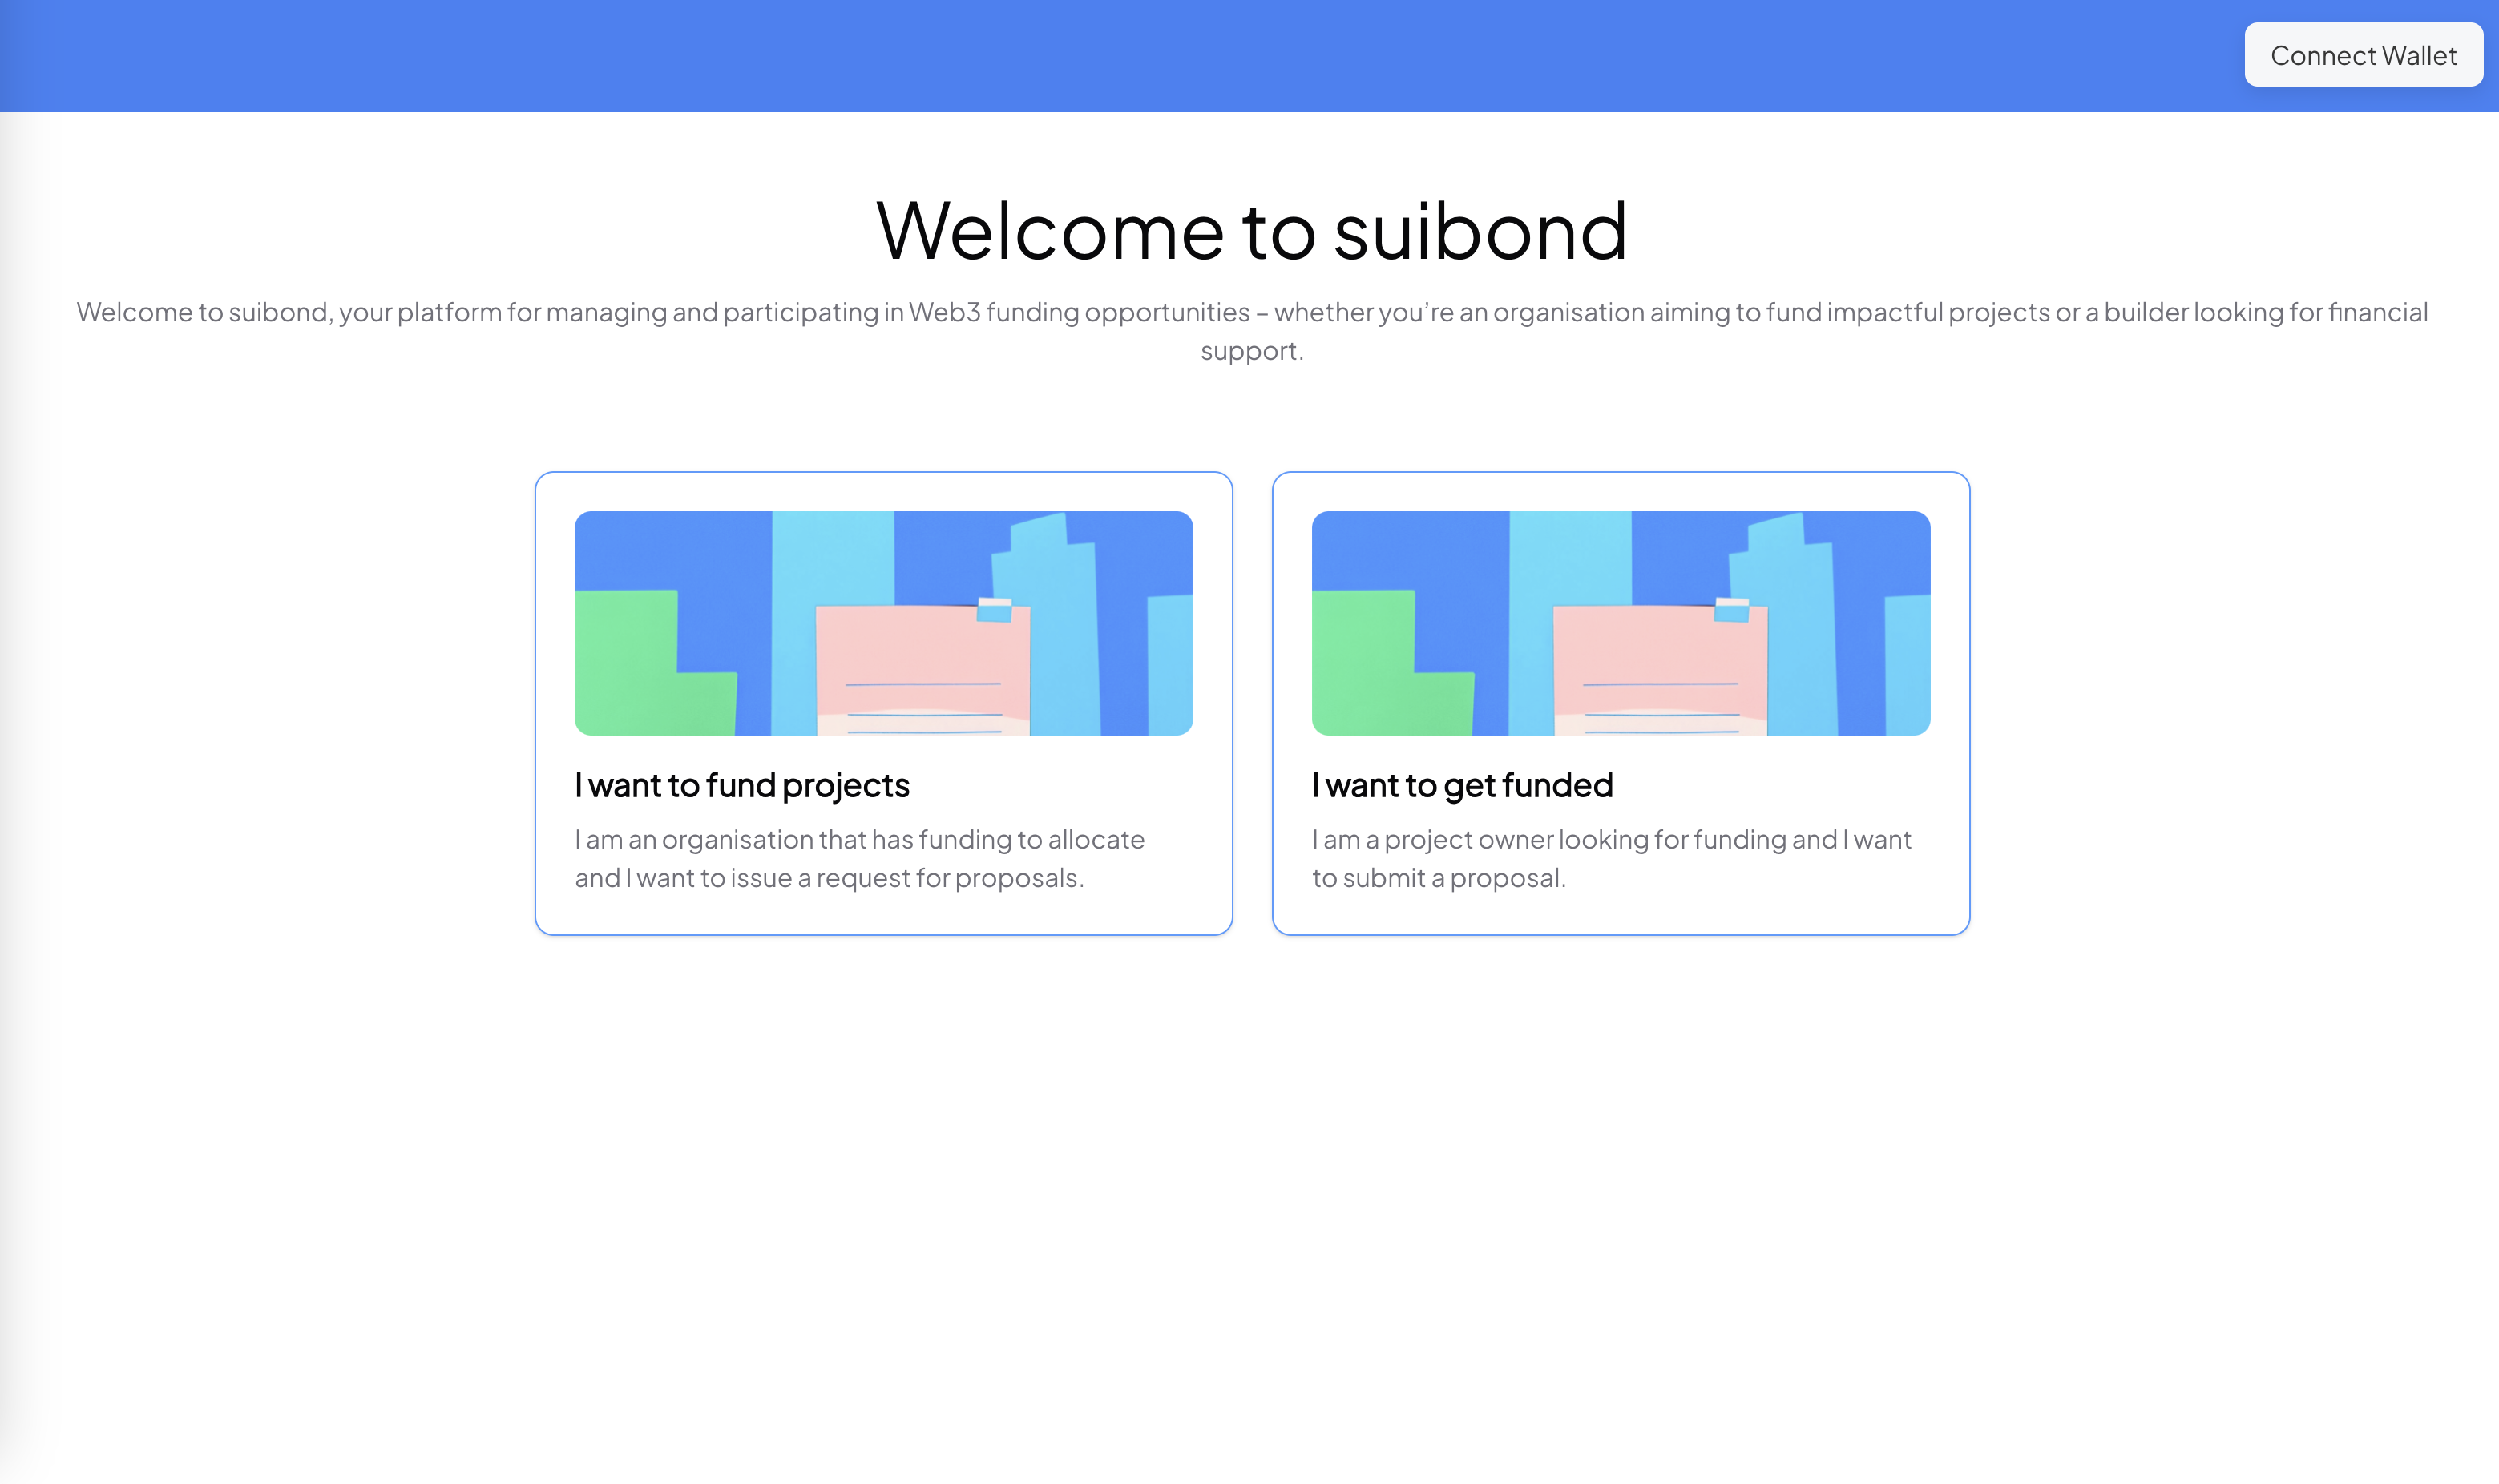
\includegraphics[scale=0.1]{suibond.png}}
\caption{This shows the suibond application.}
\label{fig}
\end{figure}


\section*{Acknowledgment}

We thank Eugene and Matthew for review and contributions.

\bibliographystyle{IEEEtran}
\bibliography{IEEEabrv,ieee_icbc_tc_bib}



\end{document}
